\subsection{Encryption and decryption}

Encryption is the transformation of message bits (\textit{plaintext}) into unintelligible form (\textit{ciphertext}) using mathematical formulas (encryption algorithm).
Only the intended recipient with the decryption algorithm can decrypt the ciphertext to see the original message \cite{Devi_2019}.
Figure \ref{fig:encryption-process.png} shows the encryption and decryption process.

\begin{figure}[!ht]
    \centering
    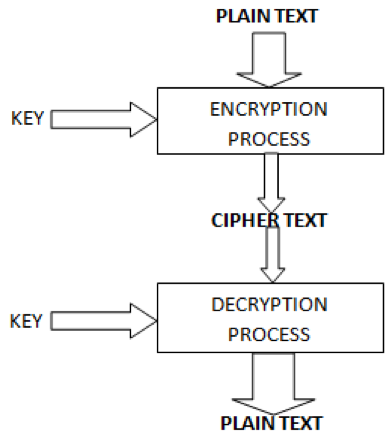
\includegraphics[width=.35\textwidth]{encryption-process.png}
    \caption{Encryption and decryption process \cite{Bhanot_2015}.}
    \label{fig:encryption-process.png}
\end{figure}


\subsubsection{Symmetric encryption}

Symmetric encryption algorithms use a single key that both the sender and recipient have.
This key is kept secret among sender and receiver so that no intruder can steal the data to be transferred by encrypting it  \cite{Bhanot_2015}.


\subsubsection{Asymmetric encryption}

Asymmetric encryption algorithm or public-key systems use two keys: a public key and a private key.
The public key is known to everyone while the private key is only used by the recipient of messages \cite{Bhanot_2015}.

Asymmetric encryption provides more security as compared to symmetric key encryption.
However, in case of encryption speed, symmetric encryption is on the lead \cite{Bhanot_2015}.

